\section{Introduction}\label{Se:introduction}
A race occurs when two concurrent threads access the same variable and when (i) at least one access is a write, (ii) the threads take no explicit mechanism to prevent the accesses from being simultaneous~\cite{eraser}. More intuitively, a race occurs when two accesses of the same variable (one is write) can happen in parallel.  Race detection is a fundamental analysis for concurrent programs, which underlies  many client applications including the atomicity/order violation detection~\cite{learning,avio,ordervio}, the dataflow analysis~\cite{dataflow} and the record and replay~\cite{leap,replay2012}. 


%fasttrack pldi paper claims happens-before analysis never reports false positives. Check it,
Over the last decade, researchers have spent tremendous efforts on race detection and have gained relative success. 
The initial efforts center around the {\em synchronization primitives} including the locks and the scheduling control such as wait/notify and start/join. Lockset analysis, which considers only locks, produces many infeasible races that contradict the schedule control. Happens-before analysis reasons about all the primitives but imposes overly restrictive lock order constraints, i.e., two lock regions with the same lock should follow the execution order as observed. The following work further relaxes the lock constraints: Hybrid analysis allows the two lock regions to be ordered in either way; {\sf Universal Causal Graph (UCG)}~\cite{ucg} allows them to be ordered in either way only when this relaxation does not contradict the schedule control.  

However, these seminal work misses the important {\em value constraints}, leading to false positives. Consider the example in Figure~\ref{fig:running}, 
where {\tt x} and {\tt y} are shared variables and no synchronizations are employed. The work that considers only synchronization constraints would report a race between line 2 and line 5 on x, which appear in the observed run. However, the race is a false alarm because line 5 can be executed only after line 4 reads the value of {\tt y} from line 3 (after line 2). 

\begin{figure}
\centering
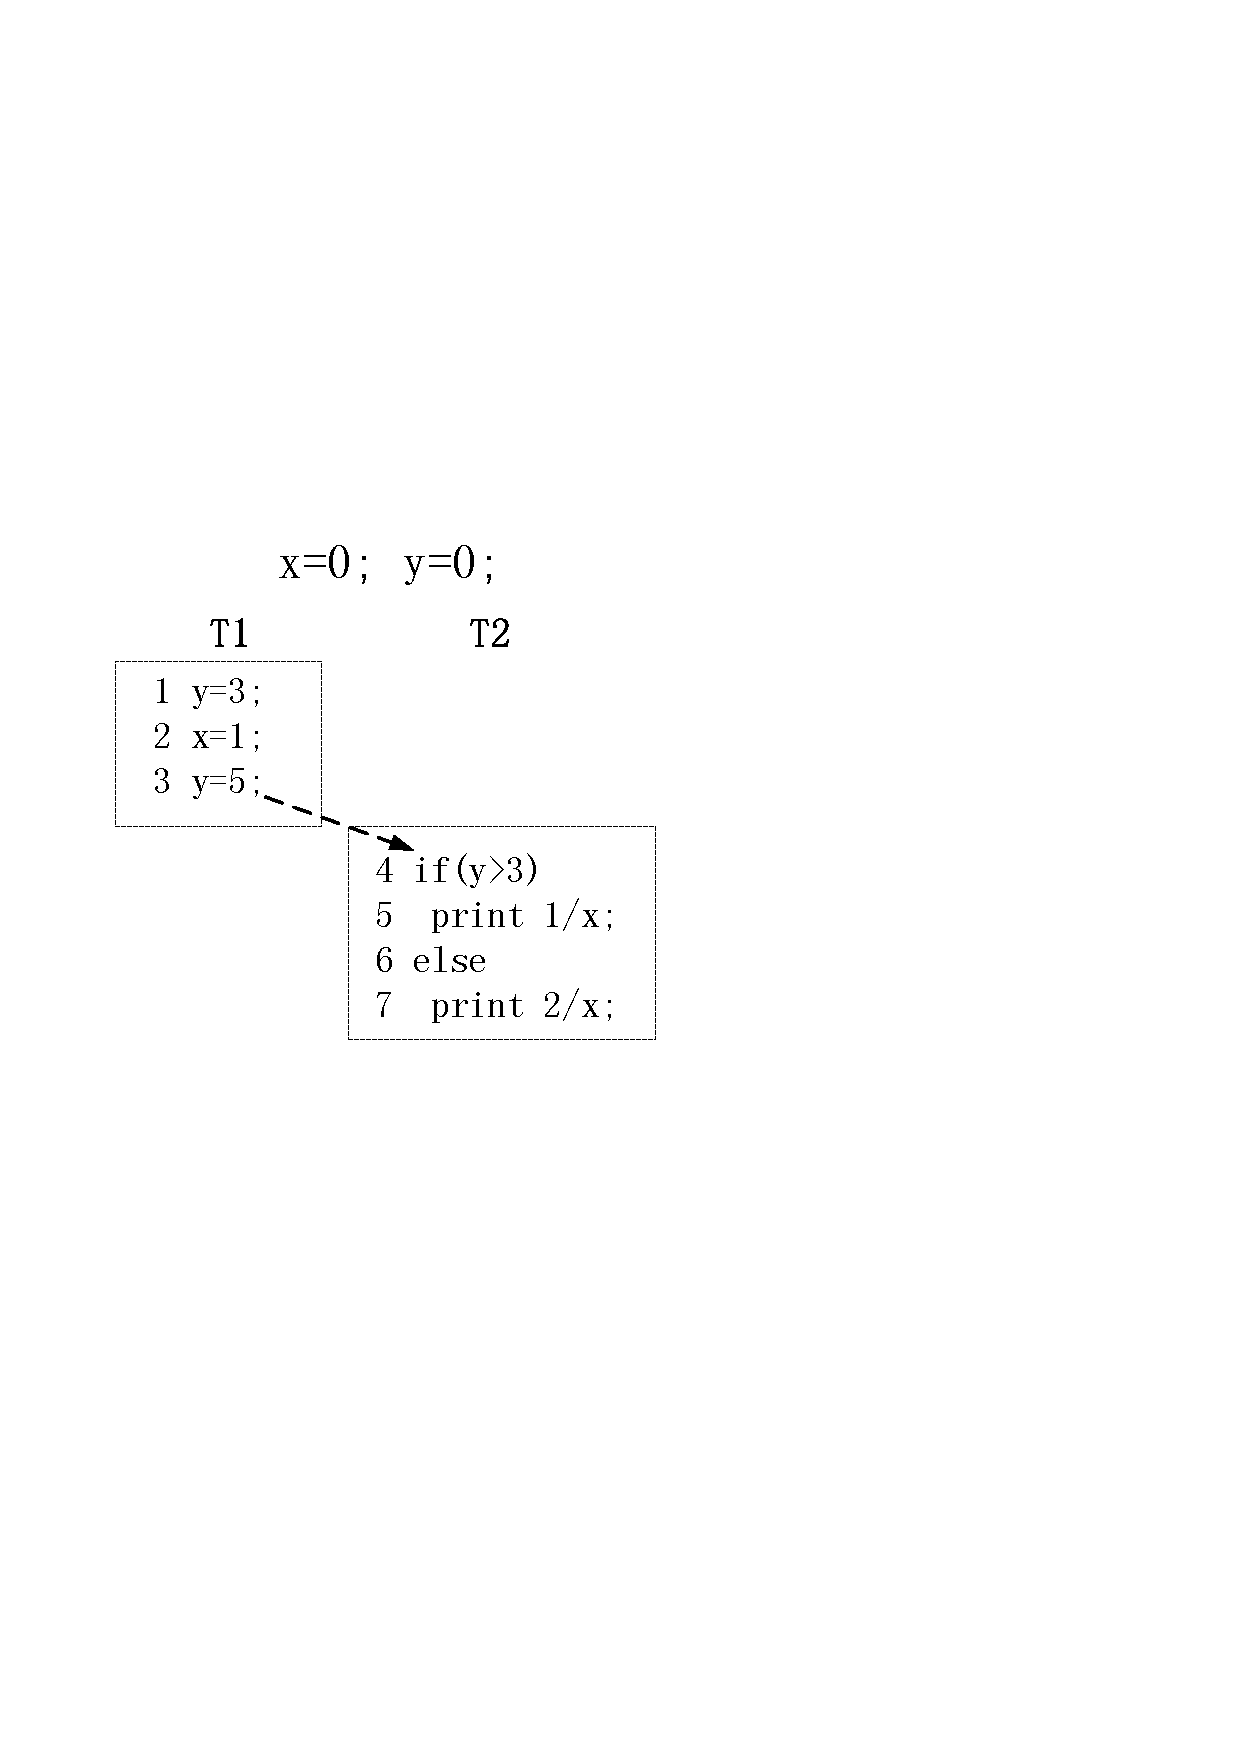
\includegraphics[width=0.38\textwidth]{figs/Visio-running.pdf}
\caption{Running Example}
\label{fig:running}
\end{figure}


%I really think Yannis' original approach is incorrect as it only preserves the dependence imposed by lock regions, which is insufficient. Check it or Hide it?
The false positives greatly reduce the usability of the detection tool as programmers need to spend great efforts  in investigating each of them. 
Recently, the predictive analysis attracts increasing research attention for its soundness guarantee, i.e., no false alarms. Smagardakis et al. pioneered by proposing first of such work. Starting from an original trace, their sound predictive analysis ``predicts'' a new trace by relaxing the execution order 
 while preserving the inter-thread dependence constraints and the synchronization constraints.  The inter-thread dependence constraints require the predicted trace and the original trace to exhibit the same set of dependences between conflicting accesses. Preservation of them leads to the soundness 
 as every value remains the same. Huang et al.~\cite{} further optimizes by preserving only the inter-thread dependences that could affect the branch decisions in the following executions.  
 
Although showing promises,  existing sound predictive analyses  are conservative as they satisfy the value constraints imposed by the branch conditions by preserving the inter-thread dependences and reading the same values at the branches. In this work, we propose the relaxed sound predictive analysis, which relaxes the value constraints to find more races without sacrificing the soundness. Our relaxation follows two key insights. First, we satisfy the value constraints computationally, rather than recording and preserving the dependences. The values read at the branches are allowed to change in the prediction as long as the change does not affect the branch decisions.  We realize the value constraints through  the satisfiability checker. Second, even if the change of the read values affects the branch decisions, we can still explore the un-executed branch  if it is ``simple'' enough. The underlying rationale is, when the executed branch contains the shared accesses, the sibling (un-executed) branch is likely to access the same shared variable. Reasoning about the un-executed branch is enabled by flexibility of  our computation-based approach, i.e., we just need to reverse the branch condition and resend it to the checker, while existing approaches cannot support such reasoning due to the lack of the computation power and the conservativeness of perservation-based approaches. 


We highlight our approach with the example~\footnote{We omit the synchronization primitives purposely for simplification.} in Figure~\ref{fig:running}. Suppose the branch at line 4 changes to {\tt if(y>=3)}. In the original run, line 4 reads from the value defined at line 3. Therefore, Huang et al.'s approach preserves the same dependence in the predicted run, and therefore misses the race on x between line 2 and line 5. In contrast, our approach reports two more real races on x, (2,5) and (2,7). 

We first demonstrate how we find the race (2,5). As shown in Figure~\ref{fig:demo}, we first encode trace in the SSA form, where each variable is defined exactly once (line number as the superscript). Besides, we introduce a new symbol, e.g., $R^4_{y}$,  to denote each shared read, e.g., the read of $y$ at   
 line 4. We also list the constraints for a valid predicted run. Race constraints specify line 2 and line 5 can run in parallel. Here $O_2$ and $O_5$ are  variables introduced to denote the orders. Program order constraints specify the intra-thread execution order. The rest  constraints model the value constraints: path condition constraints specify the branch decision for the branches preceding the potential racy event line 5; variable definition 
 constraints specify the intra-thread value flow due to each assignment; Inter-thread constraints specify the inter-thread value flow which is conditioned on the scheduling constraints. For example, $R^4_{y}=y^1 \wedge O_1< O_4 <O_3$ specifies that line 4 reads {\tt y} defined at line 1 if and only if line 4   
  happens after line 1 and before line 3.  Combined together, the constraints are sent to off-the-shelf solver such as z3 or yices, which then returns a solution: line 4 reads $y$ ($y$=3) defined at line 1, which satisfies the branch condition. 
  
Finding the race (2,7) requires a slightly different set of constraints. Specifically, the race constraint becomes $O_2=O_7$, and the path condition constraint becomes $R^4_y<3$. The checker also returns a solution for these constraints: line 4 reads $y$ ($y$=0) from the initial value, which steers the execution towards the unexecuted path at the branch line 4.

  
  

\begin{figure}
\centering
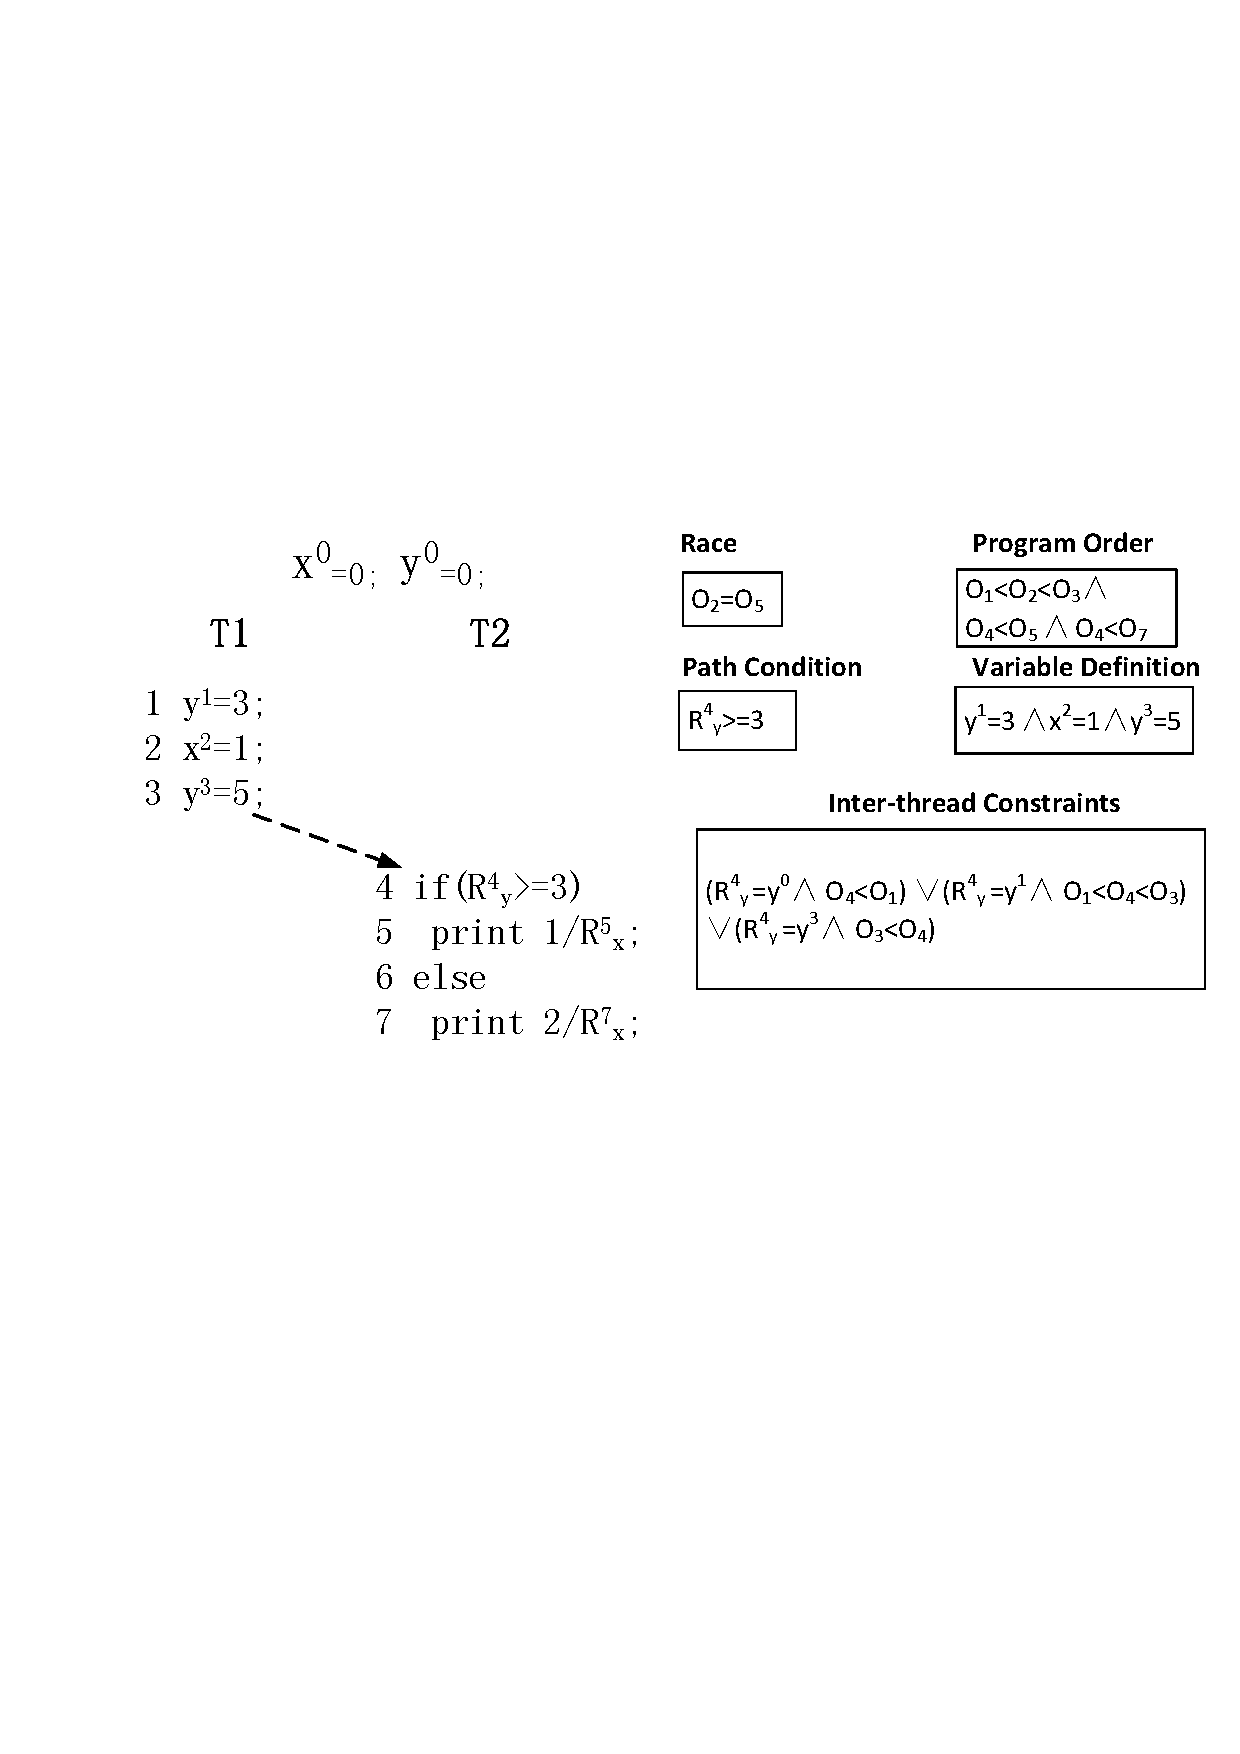
\includegraphics[width=0.5\textwidth]{figs/Visio-demo.pdf}
\caption{Overview}
\label{fig:demo}
\end{figure}






\paragraph{Contributions} The principal contributions of this paper are the following:
